\section{ Don't you see!}

\parpic[r]{
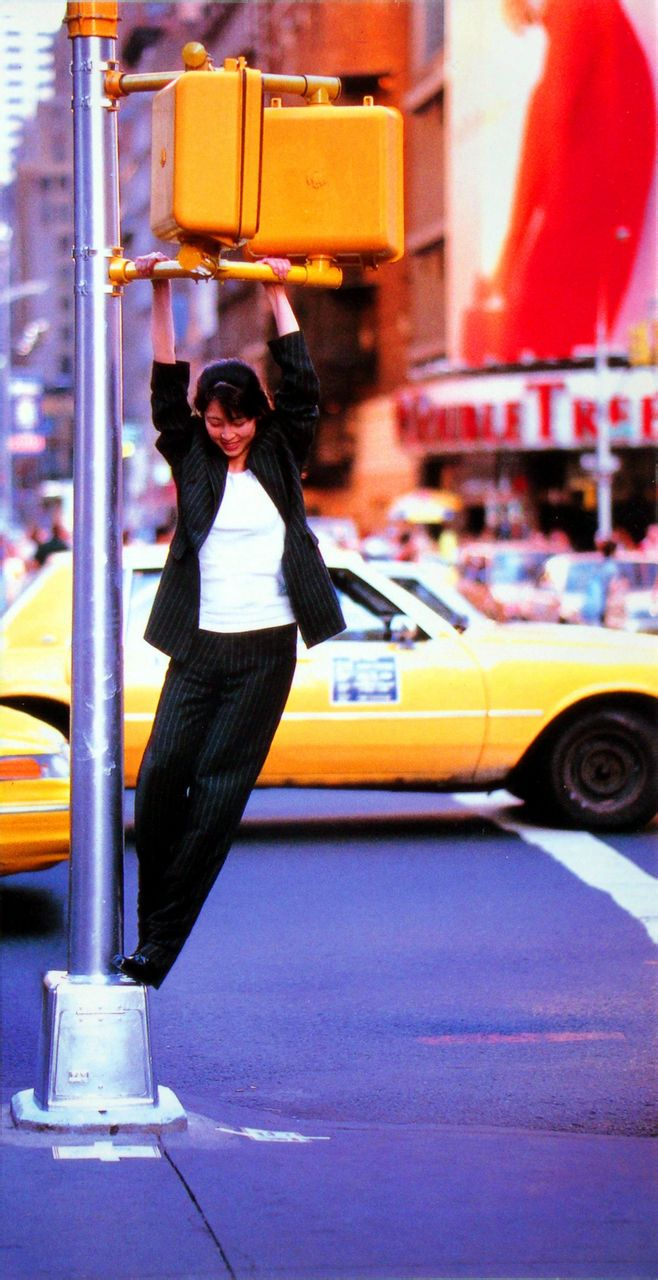
\includegraphics[width=0.3\textwidth]{S19.jpg}}

\large{

\ruby{友達}{ともだち}に\ruby{手紙}{てがみ}を\ruby{書}{か}くときみたいに

スラスラ\ruby{言葉}{ことば}が\ruby{出}{で}てくればいいのに

もう\ruby{少}{すこ}しお\ruby{互}{たが}いを\ruby{知}{し}り\ruby{合}{あ}うには 

\ruby{時間}{じかん}が\ruby{欲}{ほし}しい

\ruby{裏切}{うらぎ}らないのは \ruby{家族}{かぞく}だけなんて

\ruby{寂}{さび}しすぎるよ Love is asking to be loved

\ruby{信}{しん}じる\ruby{事}{こと}を\ruby{止}{や}めてしまえば 

\ruby{楽}{らく}になるってわかってるけど

   

Don't you see!

\ruby{願}{ねが}っても\ruby{祈}{いの}っても

\ruby{奇跡}{きせき} \ruby{思}{おも}い\ruby{出}{だ}  \ruby{少}{すこ}しは\ruby{気}{き}にかけて

Don't you see! 

ちょっと\ruby{醒}{さ}めたふりをするクセは

\ruby{傷}{きず}つくのが\ruby{怖}{こわ}いから 
\\

\ruby{TAXI乗}{の}り\ruby{場}{ば}で  \ruby{待}{ま}ってた\ruby{時}{とき}の\ruby{沈黙}{ちんもく}は

たった\ruby{5分}{ごふん}なのに ものすごく\ruby{長}{なが}く\ruby{感}{かん}じた

\ruby{無理}{むり}をして \ruby{疲}{つか}れて 

\ruby{青}{あお}ざめた\ruby{恋}{こい}は\ruby{予期}{よき}せぬ\ruby{出来事}{できごと}
\\

Don't you see! 

\ruby{小}{ちい}さなケンカで

\ruby{負}{ま}けず\ruby{嫌}{きら}いな\ruby{二人}{ふたり}だから ホッとしたの

Don't you see!

いろんな\ruby{人}{ひと}を\ruby{見}{み}るより

ずっと\ruby{同}{おな}じあなたを\ruby{見}{み}ていたい
\\

Don't you see! 

I'll never worry, tonight.

I'll lay me down, tonight.

You know, I do it for you.
\\

Don't you see! 

\ruby{生}{う}まれた\ruby{街}{まち}の\ruby{匂}{にお}い

\ruby{暮}{く}れかかる\ruby{街路樹}{がいろじゅう}を\ruby{二人}{ふたり}\ruby{歩}{ある}けば

Don't you see!

\ruby{世界中}{せかいじゅう}の\ruby{誰}{だれ}もが 

どんなに\ruby{急}{いそ}いでも

\ruby{私}{わたし}をつかまえていて

}